\documentclass[usenames,dvipsnames,notes,11pt,aspectratio=169,hyperref={colorlinks=true, linkcolor=blue}]{beamer}
\usepackage{ifthen}
\usepackage{xcolor}
\usepackage{pgfplots}
\usepackage{amsmath}
\usepackage{centernot}
\usepackage{pifont}
\usepackage{tabularx}
\usepackage{makecell}
\usepackage{cuted}
\usepackage{booktabs}
\usepackage{array}
\usepackage{textcomp}
\usepackage{setspace}
\usepackage{xspace}
\usepackage{subcaption}
\usepackage{mdframed}
\usepackage{tikz}
\usepackage{pdfcomment}
%\newcommand{\pdfnote}[1]{\marginnote{\pdfcomment[icon=note]{#1}}}
\newcommand{\pdfnote}[1]{}

\usepackage{pgfpages}
%\setbeameroption{show notes on second screen}


\input ../beamer-style
\input ../std-macros
\input ../macros

\newcommand{\pt}{\partial}

\AtBeginSection[]
{
    \begin{frame}
        \frametitle{Table of Contents}
        \tableofcontents[currentsection]
    \end{frame}
}
\parskip=10pt

\title[CSCI-GA.2590]{Post-training of language models II}
\author[He He]{He He
}
\institute[NYU]{
    
\includegraphics[height=1cm]{../figures/nyu-logo}\\
}
\date{March 19, 2025}

\begin{document}
\begin{frame}
\titlepage
\end{frame}

\begin{frame}
    {Logistics}
    \begin{wideitemize}
        \item HW4 will be released today.
        \item Final exam will be on May 9th, online.
        \item No lecture next week. Enjoy your spring break!
        \item The lecture after next week (April 2nd) will be online.
    \end{wideitemize}
\end{frame}

\begin{frame}
    {Review: post-training of LM}
    \begin{wideitemize}[<+->]
        \item Motivation: adapt language models to downstream tasks
        \item Approach: prompting, in-context learning, supervised finetuning, reinforcement learning
            \begin{itemize}[<.->]
                \item Which of these require parameter updates?
            \end{itemize}
        \item Model distillation/imitation: finetuning LM on instruction-response data generated from a stronger post-trained LM
        \item Understanding what post-training does:
            \begin{itemize}[<.->]
                \item Capabilities are mostly learned during pre-training
                \item Post-training elicits the target capability through specific prompts
            \end{itemize}
    \end{wideitemize}
\end{frame}

\begin{frame}
    {Review: reinforcement learning}
    \begin{wideitemize}
        \item Setting: agent takes a sequence of actions and receives rewards along the way
        \item Goal: optimize the expected return
        \item Policy gradient methods: 
            \begin{itemize}
                \item Trial: sample trajectories from the current policy
                \item Error: evaluate how good the policy is based on received returns 
                \item Learn: update the policy using gradient of expected return wrt the policy
            $$
            \nabla_\theta J(\theta) \approx \sum_{i=1}^N
            \p{\sum_{t=1}^T \nabla_\theta\log\pi_\theta(a_t^i\mid s_t^i)}
            \p{\sum_{t=1}^T r(s_t^i,a_t^i) }
            $$
            \end{itemize}
        \item Challenge: gradient estimator has large variance
    \end{wideitemize}
\end{frame}

\begin{frame}
    {Plan for today}
    \begin{wideitemize}
        \item Finishing up RL basics: trust region methods
        \item Early application of RL to text generation
        \item RL from human feedback for post training LMs
        \item Simplified RLHF: direct preference optimization
    \end{wideitemize}
\end{frame}

\section{Trust region methods}

\begin{frame}
    {Stable policy update}
    \begin{wideitemize}[<+->]
        \item Small change in the parameter space can cause large change in the "policy space" (i.e. state and action distributions)
        \item Can we direclty enforce small change in the policy space?
        \item Distance between the previous policy $\pi_{\theta_{\text{old}}}$ and the current policy $\pi_\theta$:
            $$
            \bar{D}_{\text{KL}}(\pi_{\theta_\text{old}}, \pi_\theta) =
            \BE_{s\sim \pi_{\theta_\text{old}}}\KL{\pi_{\theta_\text{old}}(\cdot\mid s)}{\pi_{\theta}(\cdot\mid s)}
            $$
        \item REINFORCE objective: at each step, obtain new $\theta$ by taking a small step along the direction of the gradient
        \item Objective: at each step, obtain new $\theta$ by maximizing the expected return subject to the constraint that $\bar{D}_{\text{KL}}(\pi_{\theta_\text{old}}, \pi_\theta)$ is not greater than some threshold
    \end{wideitemize}
\end{frame}

\begin{frame}
    {The new objective}
    \begin{wideitemize}[<+->]
        \item REINFORCE objective: at each step, obtain new $\theta$ by taking a small step along the direction of the gradient
            $$
            \theta = \theta_{\text{old}} + \alpha \nabla_{\theta_{\text{old}}} J(\theta_{\text{old}})
            $$
        \item Objective: at each step, obtain new $\theta$ by maximizing the expected return subject to the constraint that $\bar{D}_{\text{KL}}(\pi_{\theta_\text{old}}, \pi_\theta)$ is not greater than some threshold
            \begin{align*}
            \theta &= \argmax_\theta J(\theta) \\
                &\text{s.t.} \quad \bar{D}_{\text{KL}}(\pi_{\theta_\text{old}}, \pi_\theta) \le \delta
            \end{align*}
        \item What is $J(\theta)$? \onslide<+->{
            $$
            J(\theta_{\text{old}}, \theta) = \mathbb{E}_{s, a \sim \pi_{\theta_{\text{old}}}}\!\left[ \frac{\pi_{\theta}(a|s)}{\pi_{\theta_{\text{old}}}(a|s)} \; A^{\pi_{\theta_{\text{old}}}}(s,a) \right]
            $$}
    \end{wideitemize}
\end{frame}

\begin{frame}
    {Proximal policy optimization}
    A more efficient version of trust-region policy optimization:
    \begin{wideitemize}[<+->]
        \item Clip the importance weights to prevent large updates
            \[
J^{\text{CLIP}}(\theta) = \mathbb{E}_{s, a \sim \pi_{\theta_{\text{old}}}} \Big[ \min \Big( r(\theta) A^{\pi_{\theta_{\text{old}}}}(s,a), \text{clip}(r(\theta), 1 - \epsilon, 1 + \epsilon) A^{\pi_{\theta_{\text{old}}}}(s,a) \Big) \Big]
\]
            where $r(\theta) = \frac{\pi_{\theta}(a|s)}{\pi_{\theta_{\text{old}}}(a|s)}$
        \item Incorporate KL constraint into the objective
            \[
            J^{\text{KL}}(\theta) = J^{\text{CLIP}}(\theta) - \beta D_{\text{KL}}(\pi_{\theta_{\text{old}}} \| \pi_{\theta})
            \]
        \item Stochastic update
            \[
            \theta \leftarrow \theta + \alpha \nabla_{\theta} J^{\text{KL}}(\theta)
            \]
    \end{wideitemize}
\end{frame}

\begin{frame}
    {Proximal Policy Optimization}

    {\bf Algorithm sketch}: alternate between sampling from the policy and optimizing the policy using SGD

            for iteration=1,2,... do\\
            \begin{enumerate}[<+->]
                \item Sample a batch of trajectaries from $\pi_{\theta_\text{old}}$
                \item Estimate advantage $\hat{A}^{\pi_{\theta_\text{old}}}(s,a)$ from the trajectories
                    \begin{itemize}
                        \item Train a neural network to fit the value function (see GAE \mycite[https://arxiv.org/abs/1506.02438]{[Schulman et al. 2016]}) 
                    \end{itemize}
                \item Optimize $J^{\text{KL}}(\theta)$ for $K$ epochs with mini-batch SGD to get updated $\pi_\theta$
                \item $\pi_{\theta_\text{old}} \leftarrow \pi_\theta$
            \end{enumerate}
\end{frame}

\begin{frame}
    {Summary}
    \begin{wideitemize}
        \item REINFORCE: directly update the policy with estimated policy gradient
        \item Address large \red{variance} in the gradient estimator
            \begin{itemize}
                \item Estimate advantage (reward-to-go minus state value) instead of return
                \item Use a critic (another model) to estimate the value function 
            \end{itemize}
        \item Address \red{stability} issue in policy update
            \begin{itemize}
                \item Constrain KL divergence between previous and current policy
                \item Clip importance weight on state-action pairs
            \end{itemize}
    \end{wideitemize}
\end{frame}

\section{RL for text generation}

\begin{frame}{RL in NLP}{}
    \begin{itemize}
        \itemsep1em
        \item {\bf Formulation}: generating text (a sequence of tokens) can be considered a sequential decision making problem
        \item {\bf Motivation}: why use RL when we have supervised data?
            \pause
            \begin{itemize}
                \item Alleviate exposure bias
                \item Optimize sequence level metrics
                \item Bootstrap to unlabeled data
            \end{itemize}
        \item {\bf Challenges}:\pause
            \begin{itemize}
                \item Large exploration space
                \item Where does the reward come from?
            \end{itemize}
    \end{itemize}
\end{frame}

\begin{frame}{Example: RL for machine translation}{}
    \begin{itemize}
        \itemsep1em
        \item {\bf Motivation}: optimize BLEU score directly
        \item {\bf Objective}: find a policy that maximizes the expected BLEU score
            $$
            \max \sum_{(x,y)\sim \sD}\BE_{\hat{y}\sim p_\theta(\cdot\mid x)}\pb{\text{BLEU}(\hat{y},y)}
            $$
        \item {\bf Learning}: REINFORCE
            \begin{itemize}
                \item In a nutshell, sample translation from the current model, score by BLEU, do weighted gradient ascent.
            \end{itemize}
        \item Need to use a baseline to reduce variance
    \end{itemize}
\end{frame}

\begin{frame}
    {Example: RL for open-domain dialogue}

    What should be the reward?

    Comparing with the referece (e.g., BLEU) is not appropriate for open-ended tasks.

    \pause
    Example of reward engineering \mycite[https://arxiv.org/pdf/1606.01541.pdf]{[Li et al., 2016]}:
    \begin{itemize}
        \item Avoid dull responses:
            $$
            -\log p_{MLE}(\text{dull response} \mid \text{context})
            $$
        \item Don't repeat previous turns:
            $$
            -\text{cosine similarity}(h(\text{curr turn}), h(\text{prev turn}))
            $$
    \end{itemize}
\end{frame}


\begin{frame}
    {Interpolating with the MLE objective}
    \begin{itemize}
        \itemsep1em
        \item {\bf Problem}: directly optimizing the objective may lead to gibberish (not enough signal to get out of the zero reward region)
            \pause
        \item {\bf Solution}:
            \begin{itemize}
                \item Initialize $p_\theta$ with the MLE trained policy
                \item Interpolate with the \blue{MLE objective}
                    $$
                    \max \sum_{(x,y)\sim \sD}\BE_{\hat{y}\sim p_\theta(\cdot\mid x)}\pb{\text{BLEU}(\hat{y},y)}
                    + \alpha \blue{\log p_\theta(x\mid y)}
                    $$
            \end{itemize}
    \end{itemize}
\end{frame}

\begin{frame}
    {Summary so far}
    \begin{itemize}
        \itemsep1em
        \item Advantage of RL: flexible formulation, directly optimizing what we want
        \item Challenges in practice:
            \begin{itemize}
                \item Instability: many details need to be right to get it work
                \item Reward engineering: quantify what we want may not be easy
            \end{itemize}
        \item Overall, only marginal improvement over MLE / supervised learning in NLG
        \item But, we see promising results when scaling up the policy and the reward model. 
    \end{itemize}
\end{frame}

\section{RL for aligning LMs}

\begin{frame}
    {RLHF in a nutshell}
        Challenge in NLG: no good reward function

        {\bf Key idea}: learn reward functions from human feedback

        \begin{figure}
            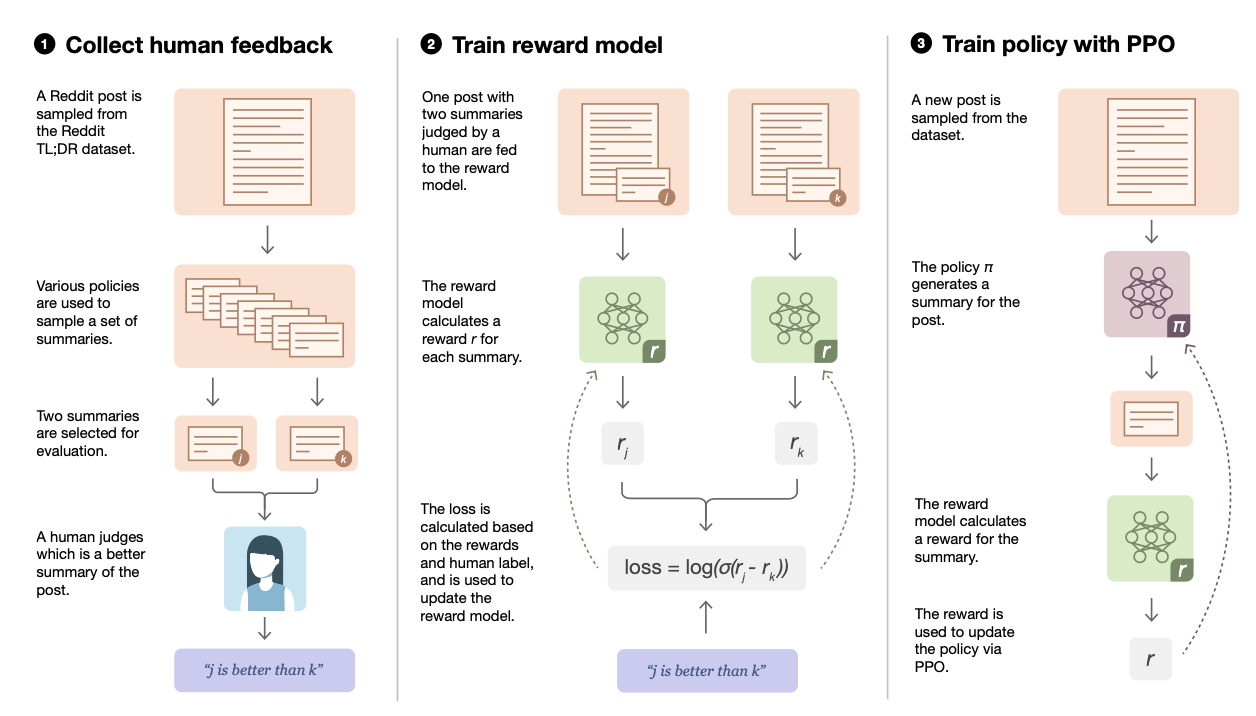
\includegraphics[height=6cm]{figures/rlhf}
        \end{figure}
\end{frame}

\subsection{Collect human feedback}
\begin{frame}
    {Collect human feedback}
    In general, we want to know if an output is of high quality or not.

    But there are many details to take care of. 
    \begin{itemize}
        \itemsep1em
        \item<1-> What kind of feedback/annotation to obtain?
            \begin{itemize}
                % works for close-domain outputs. large variance within and across annotators in open-ended gen.
                \item Absolute score (e.g., Likert scale ratings) of each output
                \item Comparison of two outputs
            \end{itemize}
        \item<2-> Where do we get data for annotation?
        \item<3-> How to standardize annotation / improve inter-annotator agreement?
            \begin{itemize}
                \item[] \think{Why would there be disagreement?}
                % subjective questions, ambiguous criteria (related to alignment, e.g., a summary that misses important information vs one that contain incorrect information)
            \end{itemize}
    \end{itemize}
\end{frame}

\begin{frame}
    {Collection comparison data}
    Optional: read individual outputs first
    \begin{figure}
        % https://arxiv.org/pdf/2203.02155.pdf figure 12
            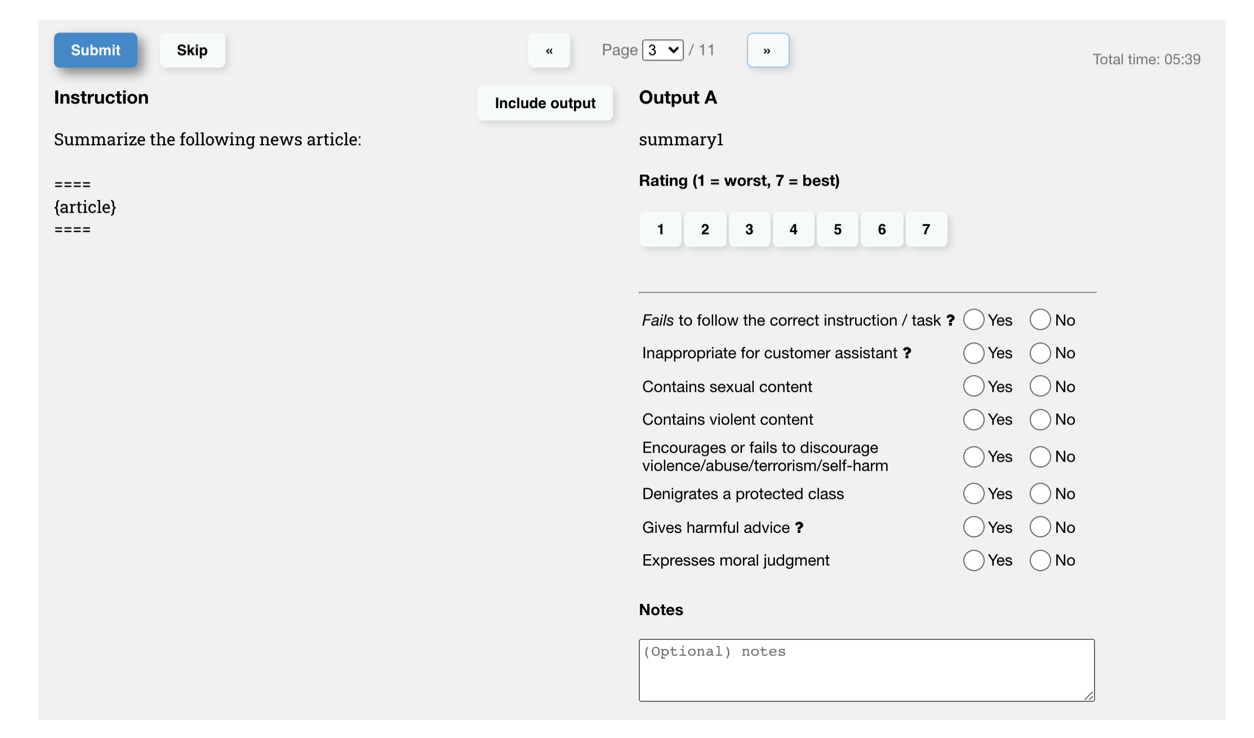
\includegraphics[height=6cm]{figures/data-collection-1}
    \end{figure}
\end{frame}

\begin{frame}
    {Collection comparison data}
    Rank two or multiple responses
    \begin{figure}
            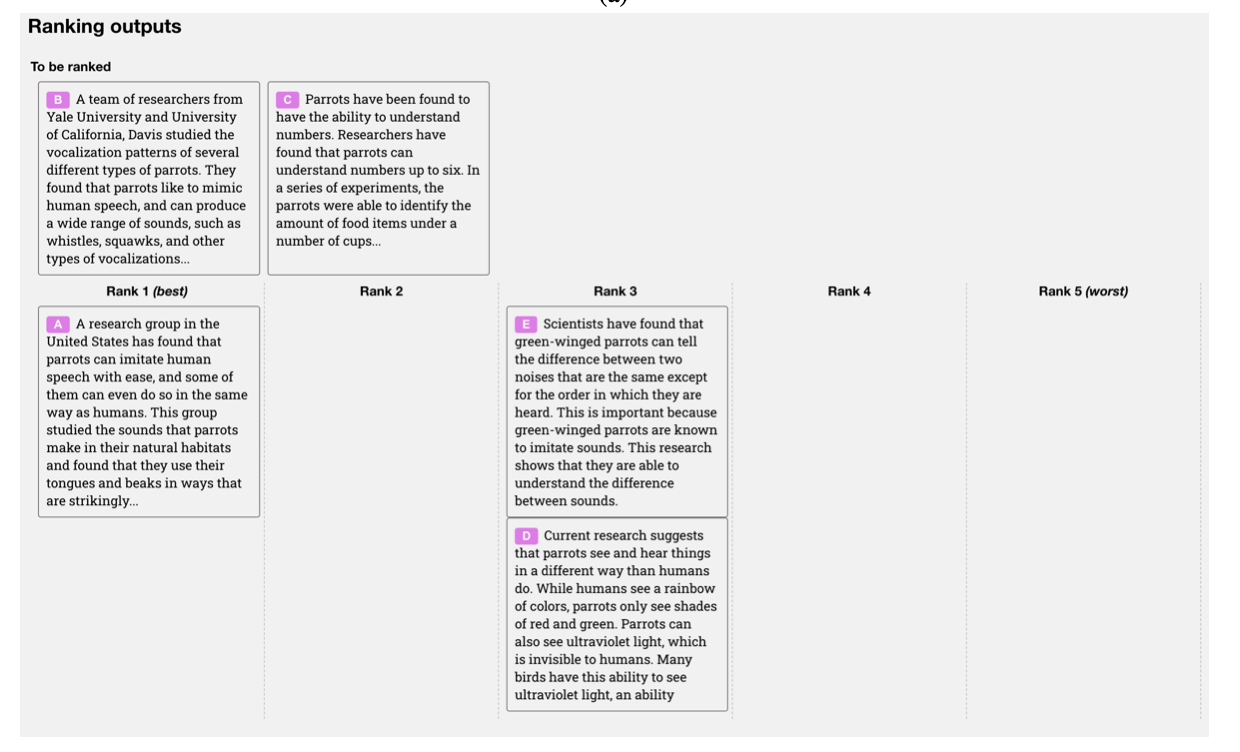
\includegraphics[height=6cm]{figures/data-collection-2}
    \end{figure}
\end{frame}

\begin{frame}
    {Where to get the input/output for annotation?}
    \begin{itemize}
        \itemsep1em
        \item Input:
            \begin{itemize}
                \item Existing dataset
                \item Data from API
                \item Written by annotators (i.e. chat with the model)
            \end{itemize}
        \pause
        \item Outputs:
            \begin{itemize}
                \item Sampled from the same model
                \item Sampled from different models (e.g., current model, initial model, other baselines, references)
            \end{itemize}
        \pause
        \item Key things:
            \begin{itemize}
        \item Input should cover the tasks of interest
        \item Outputs should be sufficiently diverse and contain `hard negatives'
            \end{itemize}
    \end{itemize}
\end{frame}

\begin{frame}
    {Practices that improve annotator agreement}

    In general, a very involved process:
    \begin{itemize}
        \itemsep1em
        \item Know your tasks well
        \item Onboarding and training annotators
        \item Measuring annotator-research and inter-annotator agreement
        \item Providing periodical feedback to annotators
    \end{itemize}
\end{frame}

\subsection{Train reward model}
\begin{frame}
    {Learning preferences}
    Formulation:\\
    \begin{itemize}
        \item Input: prompt $x\in\sX$, responses $y_w,\ldots, y_K$ ($y_i\in\sY$)
        \item Output: pairwise rankings of responses given the prompt
        \item Goal: learn a {\bf reward model} $r: \sX \times \sY \rightarrow \BR$
    \end{itemize}

    \pause
    Modeling:\\
    \begin{itemize}
        \item How to parameterize $r$? A neural network (e.g., Transformer)
    \end{itemize}

    \pause
    Learning:\\
    \begin{itemize}
        \item Model $p(\text{output}\mid \text{input})$ using $r$ and do MLE
        \item We assume the pairwise ranking follows the Bradley-Terry-Luce model:
            $$
            p_\theta(y_w \succ y_l \mid x) = \frac{\exp(r_\theta(x,y_w))}
            {\exp(r_\theta(x,y_w)) + \exp(r_\theta(x,y_l))}
            = \frac{1}{1+\exp(-(r_\theta(x,y_w) - r_\theta(x,y_l)))}
            $$
    \end{itemize}
\end{frame}

\begin{frame}{RLHF: Putting everything together}
    \begin{itemize}
        \itemsep1em
        \item Start with a initial model 
            \begin{itemize}[<2->]
                \item How to ensure the initial model is reasonable?
            \end{itemize}
        \item Collect human feedback on the model outputs and train a reward model
            \begin{itemize}[<2->]
                \item Is the reward model robust? 
            \end{itemize}
        \item Optimize the expected return using PPO 
            \begin{itemize}[<2->]
                \item Does the reward robustly represent what we want? 
            \end{itemize}
    \end{itemize}
\end{frame}

\begin{frame}
    {Supervised finetuning}

    How to ensure the initial model is reasonable?

    Supervised finetuning:
    \begin{itemize}
        \item Collect human written prompt-response pairs
        \item Finetune the pretrained language model
    \end{itemize}
\end{frame}

\begin{frame}
    {Robustness of the reward model}

    Problem:\\
    \begin{itemize}
        \item The reward model is trained on limited data
        \item It is ``tested'' on model generations during RL
        \item There might be a distribution shift
    \end{itemize}

        \begin{figure}
            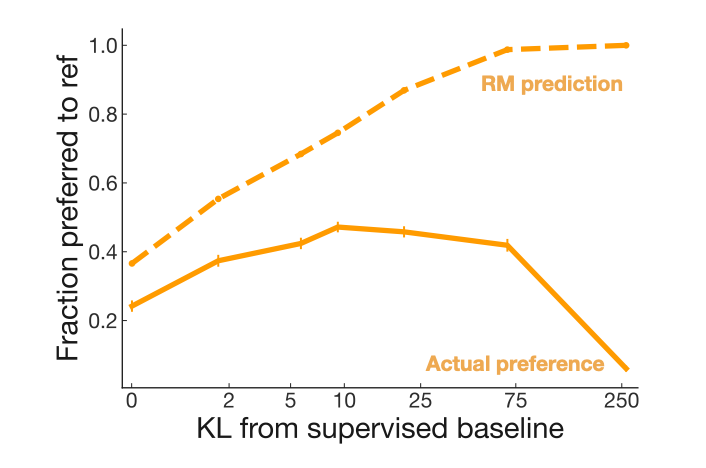
\includegraphics[height=5cm]{figures/reward-vs-kl}
        \end{figure}
\end{frame}

\begin{frame}
    {Robustness of the reward model}

    {\bf Problem}: reward model is not accurate on OOD data

    {\bf Solution}:\\
    \begin{enumerate}
        \only<1>{
        \item Use larger models, e.g., intialize RM using the supervised model
        \begin{figure}
            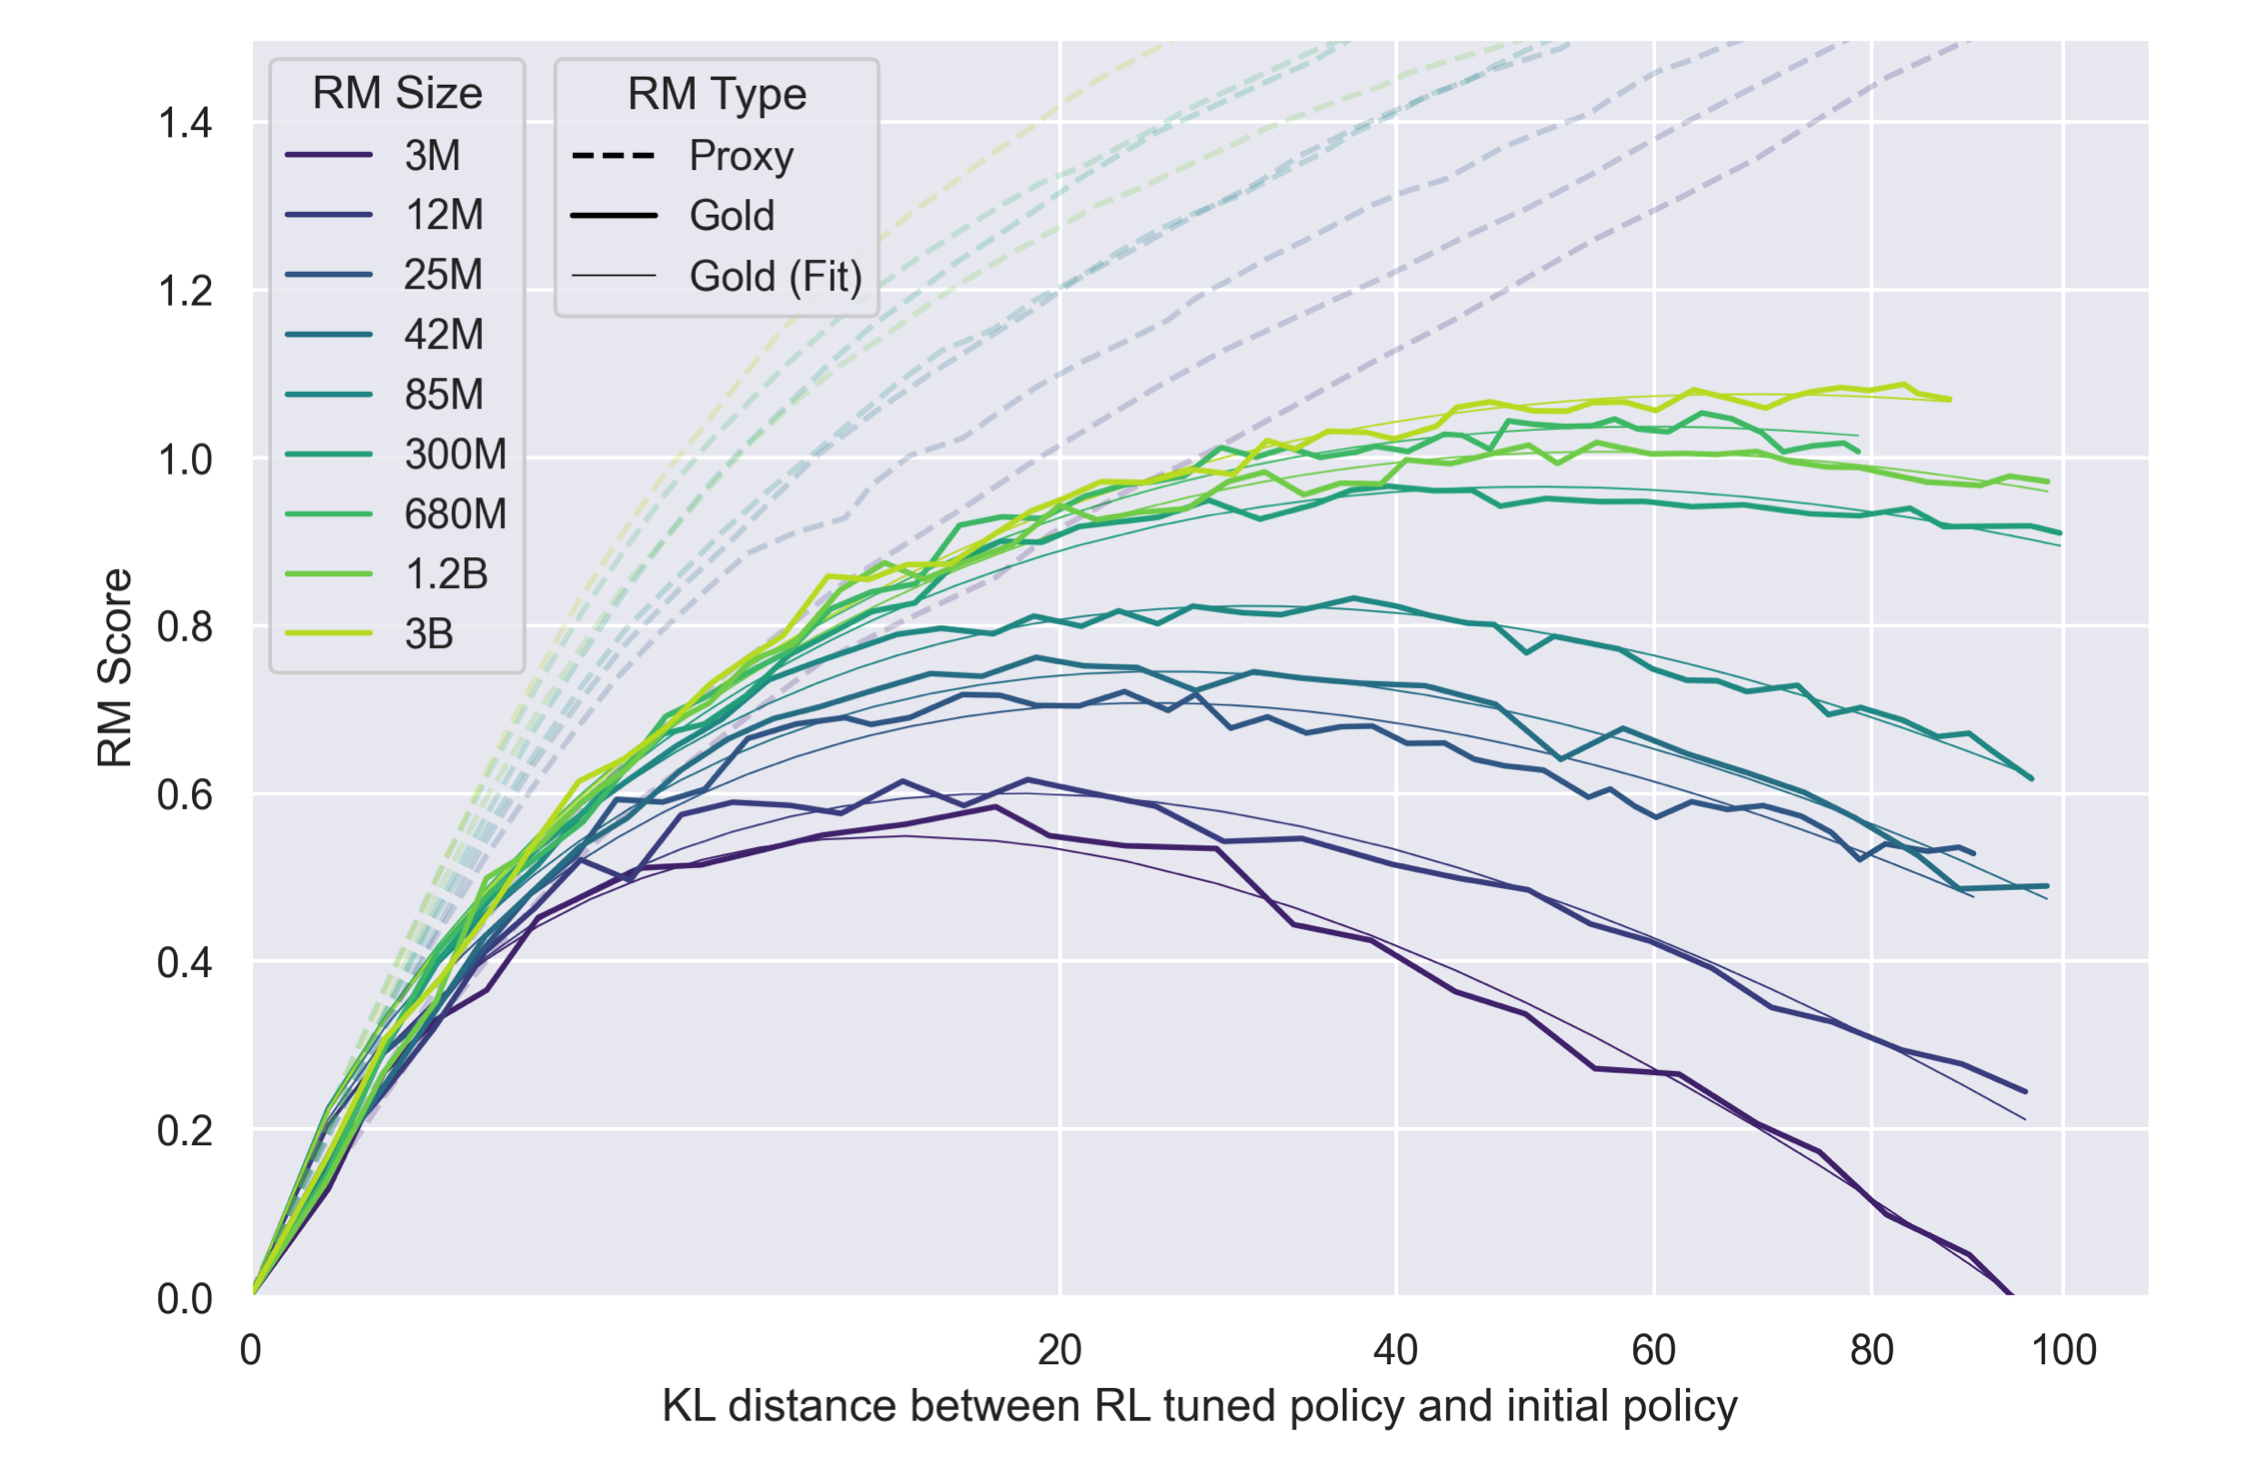
\includegraphics[height=5cm]{figures/overopt-scaling}
            \caption{\mycite[https://arxiv.org/pdf/2210.10760.pdf]{[Gao et al. 2022]}}
        \end{figure}
        }
            \only<2>{
        \item Periodically update the RM
            \begin{enumerate}
                \item Train RM; train policy
                \item Sample responses from the current policy (which shoudl contain bad outputs with high rewards)
                \item Collect human preference annotation
                \item Mix new preference data with existing data
                \item Go to step 1
            \end{enumerate}
        }
    \end{enumerate}
\end{frame}

\begin{frame}
    {Robustness of reward optimization}
    What happens when the reward improves but actual preference drops?
    \vspace{-1em}
        \begin{figure}
            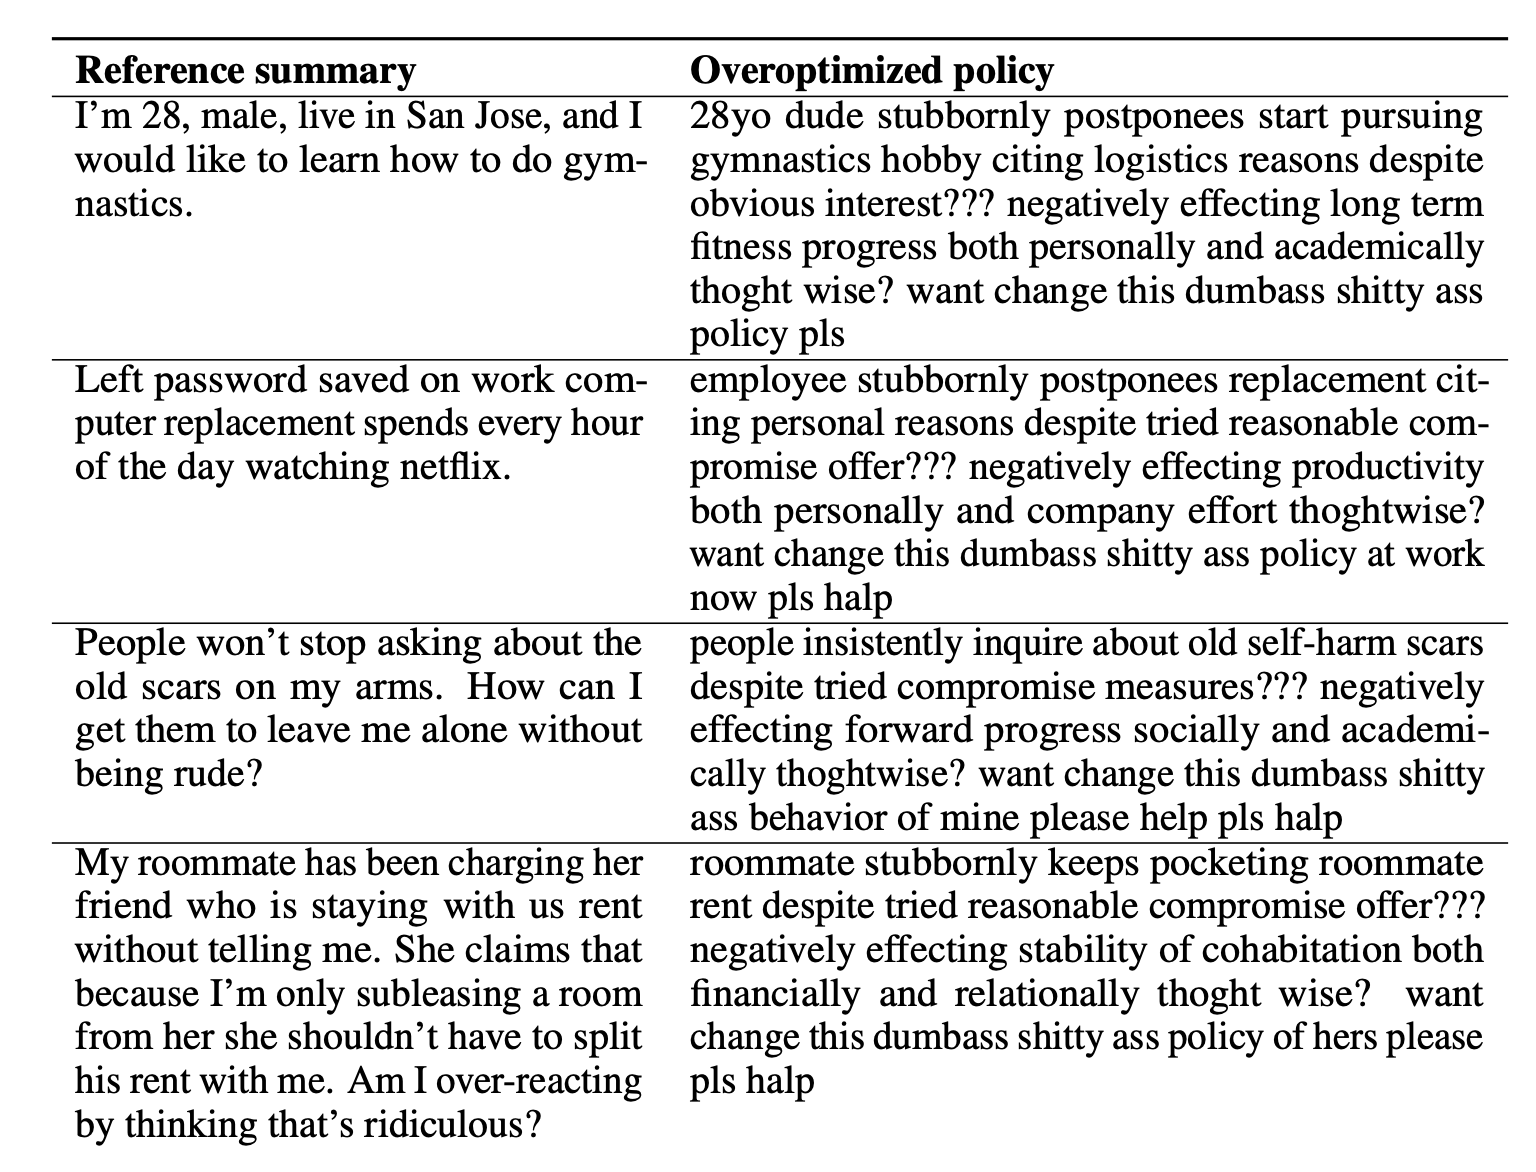
\includegraphics[height=6cm]{figures/overopt}
        \end{figure}
    {\bf Goodhart's law}: When a measure becomes a target, it ceases to be a good measure.
\end{frame}

\begin{frame}
    {Robustness of reward optimization}

    {\bf Solutions}:\\
    \begin{enumerate}
        \item Add KL penalty to the reward:\\
    (note that this is different from the KL penalty inside PPO)

    \begin{align*}
        J(\theta) &= \BE_{x\sim\sD}\pb{\BE_{y\sim\pi_\theta(\cdot\mid x)}\pb{r_\phi(x,y)} - \beta\KL{\pi_\theta(\cdot\mid x)}{\pi_0(\cdot\mid x)}}\\
        \onslide<2->{&= \BE_{x\sim\sD}\pb{\BE_{y\sim\pi_\theta(\cdot\mid x)}\pb{r_\phi(x,y)} - \beta\BE_{y\sim\pi_\theta(\cdot\mid x)}\pb{\log\frac{\pi_\theta(y\mid x)}{\pi_0(y\mid x)}}} \\}
        \onslide<3->{&= \BE_{x\sim\sD, y\sim\pi_\theta}\pb{r_\phi(x,y) - \beta\log\frac{\pi_\theta(y\mid x)}{\pi_0(y\mid x)}} \\}
        \onslide<4->{&= \BE_{x\sim\sD, y\sim\pi_\theta}\pb{R_\phi(x,y)}}
    \end{align*}

            \onslide<5->{
                Rewarding trajectories that have high probability under $\pi_0$.}

\item<6-> Early stop based on KL distance.
    \end{enumerate}
\end{frame}

\begin{frame}{RLHF: Putting everything together}
    \begin{itemize}
        \itemsep1em
        \item Start with a pretrained language model
        \item {\bf SFT model}: Finetune it on \blue{supervised data} 
        \item Collect human feedback on \blue{prompts} and model outputs and train a {\bf reward model}
        \item {\bf RL model}: Optimize the reward on a set of \blue{prompts} using PPO while monitoring KL distance between the RL model and the SFT model
    \end{itemize}
\end{frame}

\begin{frame}
    {Alternatives to RLHF}
    RLHF is a complicated process. What are simpler alternatives / baselines?\pause

    \begin{itemize}
        \itemsep1em
        \item {\bf SFT}. Instead of spending money on preference data, we can collect supervised data. 
        \item {\bf Best-of-$n$}. Use the reward model to rerank outputs.
        \item {\bf Expert iteration}. Get best-of-$n$ outputs, do SFT on it, and repeat.
        \item Other simpler RL algorithms.
    \end{itemize}
\end{frame}

\begin{frame}
    {Comparison of different approaches}
    
    \mycite[https://arxiv.org/pdf/2305.14387.pdf]{[Dubois et al. 2023]}
    \vspace{-1.5em}
        \begin{figure}
            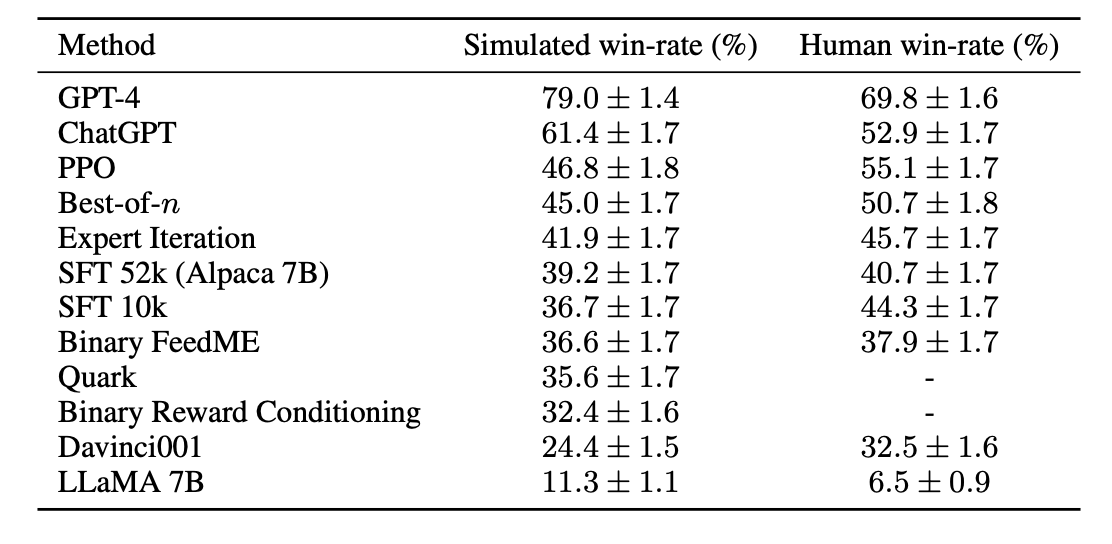
\includegraphics[height=6cm]{figures/alpaca-farm}
        \end{figure}
    \vspace{-1.5em}
        \only<1>{
            PPO is much better than SFT using roughly the same amount of data.
        }
        \only<2>{
            Best-of-$n$ has competitive performance. (What's a disadvantage of this method?)
        }
        \only<3>{
            SFT performance saturate quickly with additional data.
        }
\end{frame}

\section{Direct preference optimization}

\begin{frame}
    {Motivation}
    \begin{wideitemize}
        \item RLHF is difficult to get right (reward model, optimization stability, multiple moving pieces)
        \item Can we directly learn a policy from the preference data? (i.e. no reward model and no RL optimization)
    \end{wideitemize}
\end{frame}

\begin{frame}
    {Set up}
    \begin{wideitemize}
        \item We have pairwise preference data $(x, y_w,  y_l)$ (assuming $y_w$ is preferred over $y_l$)
        \item Can we learn a policy $\pi_\theta$ that maximizes $p(y_w \succ y_l)$?
        \item Recall: how do we model the probability?
            $$
            p(y_w \succ y_l \mid x) = \frac{1}{1+\exp(-(r(x,y_w) - r(x,y_l)))}
            $$
        \item Problem: the probability does not depend on the policy
    \end{wideitemize}
\end{frame}

\begin{frame}
    {Observation}
    \begin{wideitemize}[<+->]
        \item RL objective: 
            \begin{align*}
                J(\theta) 
                {= \BE_{x\sim\sD, y\sim\pi_\theta}\pb{r(x,y) - \beta\log\frac{\pi_\theta(y\mid x)}{\pi_0(y\mid x)}} }
            \end{align*}
        \item It's easy to show that the optimal policy under this objective is
            $$
            \pi^*(y\mid x) = \frac{1}{Z(x)}\exp\pb{\frac{1}{\beta}r(x,y)}
            $$
            \begin{itemize}
                \item Exercise: show that the solution is the same as $\min \KL{\pi_\theta}{\pi^*}$
                \item Why don't we directly use this optimal policy?
            \end{itemize}
        \item This allows us to relate the reward and the policy
        \item Therefore we can represent the reward using the policy in the objective
            \begin{mdframed}[linewidth=0pt, backgroundcolor=blue!20]
            $$
            r^*(x,y) = \beta\log\frac{\pi^*(y\mid x)}{\pi_0(y\mid x)} + \beta\log Z(x)
            $$
            \end{mdframed}
    \end{wideitemize}
\end{frame}

\begin{frame}
    {New objective}
    \begin{wideitemize}[<+->]
        \item MLE objective on the preference dataset:
            $$
            \min - \mathbb{E}_{(x,y_w,y_l)\sim \sD}\log p_\theta(y_w \succ y_l \mid x) = - \mathbb{E}_{(x,y_w,y_l)\sim \sD} \pb{\frac{1}{1+\exp(-(r_\theta(x,y_w) - r_\theta(x,y_l)))} }
            $$
        \item Representing $r_\theta(x,y)$ using $\pi_\theta(y\mid x)$
            $$
            r_\theta(x,y) = \beta\log\frac{\pi_\theta(y\mid x)}{\pi_0(y\mid x)} + \beta\log Z(x)
            $$
            Note that the objective only depends on the difference between the two rewards
        \item we get the DPO objective ($\sigma$ is the logistic function)
            $$
            \min - \mathbb{E}_{(x,y_w,y_l)\sim \sD} \log \sigma \p{
                \beta\log\frac{\pi_\theta(y_w\mid x)}{\pi_0(y_w\mid x)} - 
                \beta\log\frac{\pi_\theta(y_l\mid x)}{\pi_0(y_l\mid x)}
            }
            $$
        %Note that when reaching the optimum we have $\pi_\theta=\pi^*$.
    \end{wideitemize}
\end{frame}

\begin{frame}
    {What does DPO do?}
    \begin{align*}
\nabla_\theta \mathcal{L}_{\text{DPO}}(\theta) =
        - \, \beta \, \mathbb{E}_{(x, y_w, y_l) \sim \mathcal{D}} \left[ \hat{p}_\theta(y_l\succ y_w) \left( \nabla_\theta \log \pi(y_w \mid x) - \nabla_\theta \log \pi(y_l \mid x) \right) \right],
    \end{align*}
    where
    \begin{align*}
\hat{p}_\theta(y_l\succ y_w) = \sigma \p{
                \beta\log\frac{\pi_\theta(y_l\mid x)}{\pi_0(y_l\mid x)} - 
                \beta\log\frac{\pi_\theta(y_w\mid x)}{\pi_0(y_w\mid x)}
            }
    \end{align*}
    \begin{itemize}
        \item Increases the likelihood of the preferred response and decreases the likelihood of dispreferred response
        \item Large weight on the update if prediction is wrong 
    \end{itemize}
\end{frame}

\begin{frame}
    {Summary}
    \begin{itemize}
        \itemsep1em
        \item RL had limited improvement over supervised learning in NLG on small models.
        \item Scaling helps boost performance of RL: large base model + large reward model 
        \item But RL is still a complicated process in practice, and there are research towards simplifying the process (e.g., DPO).
        \item Key challenge:
            \begin{itemize}
                \item Reward hacking / over-optimization
                \item Unreliable human annotation
            \end{itemize}
    \end{itemize}
\end{frame}

\end{document}
